\phantomsection
\chapter{Conclusion}
\label{chap:ccl}
  
\phantomsection
\section{Theoretical framework}

\vspace{\baselineskip}
\noindent The theoretical framework on which this system is based relies on three major points: face detection, feature extraction and classification. Face detection is achieved through Viola-Jones face detection algorithm. This cascade of AdaBoost classifiers based on Haar-like features results in a strong binary classifier, composed of a chain of small weak ones. Moreover, the use of integral images enables real-time detection.
\newline

\noindent Feature extraction is performed using Local Binary Patterns, a simple but efficient texture descriptor encoding changes in micro-patterns. It outputs histograms which bin indexes are intensity values of the pixels, and bin sizes the number of pixels having this value. This texture descriptor can be used for facial feature extraction, and can be modified in order to detect patterns of various sizes and shapes, but also to reduce histogram size, hence improving computation time.
\newline

\noindent Thirdly, Support Vector Machine is used as classifier. This binary linear classifier, belonging to the supervised learning category, is based on \textit{margin maximization} and \textit{kernel functions}. Indeed, since it is a linear classifier, data has to be mapped into a higher space for the classifier to perform correctly. Four classic kernels can be used, and even combined if needed. When compared to other classification methods, SVM yields better results, which makes it a suitable choice for facial expression recognition using Local Binary Patterns.
\newline

\phantomsection
\section{Results}

\vspace{\baselineskip}
\noindent Different results are obtained based on the use of the Kinect or not.
\newline

\noindent Results obtained by using face images of the KDEF database as test set are quite good, with an accuracy rate of $ 66.67\% $. There is nevertheless an issue with the \textit{sad} emotion, which stands out because of its bad recognition accuracy. This emotion is mostly misclassified as \textit{neutral} state. Indeed these two emotions are quite similar, almost identical when it comes to feature extraction, hence the low accuracy rate.
\newline

\noindent The \textit{angry} emotion also has a below average recognition accuracy, but it is not as significant as for the \textit{sad} emotion. The reason behind this result is the same as for the \textit{sad} emotion. Since an \textit{angry} face is more distorted than a \textit{sad} face it is more easily classified correctly. The accuracy rate is thus of $ 41.67\% $ for the \textit{angry} expression,  instead of $ 8.33\% $ for \textit{sad}.
\newline

\noindent Concerning results obtained with the Kinect, the accuracy rate is significantly lower.
\newline

\phantomsection
\section{Improvements}

\subsection{Local Binary Patterns}

\vspace{\baselineskip}
\noindent One of the way to improve the LBP operator of this system is to add weights for each of the 42 regions of the face, as seen in Chapter~\ref{chap:lbp}. The LBP operator used in this system is already far from the basic LBP operator; it is a uniform circular LBP operator. Even though the results obtained with this operator are quite good with an accuracy of $ 66.67\% $, there is still room for improvement. Weighting the regions of the face will have an impact on the computed histogram, hence on the resulting feature vector ready for classification. \newline

\noindent The face image is divided in 42 regions ($ 7 $ rows $\times$ $ 6 $ columns), as seen in Chapter~\ref{chap:lbp}, and mentioned in \ref{GAN08}. The weights are however not applied in the same way as in \ref{GAN08}, but rather as in Figure~\ref{lbp_region_weight}. Figure~\ref{implementation_weight_example} shows an example of the division into regions of face images from the KDEF database that this system uses. Thus, border regions are less important than those containing the ROI of the face (eyes, nose, mouth). Figure~\ref{implementation_weight_example} shows an example of the division into regions of face images from the KDEF database used by this system.
\newline

\begin{figure}[!h]
\begin{center}
\noindent 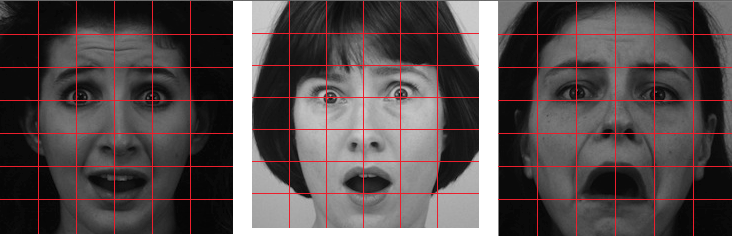
\includegraphics[scale=0.3]{figures/implementation_weight_example} 
\newline
\caption{Example of division into regions of face images from the KDEF database}
\label{implementation_weight_example}
\end{center} 
\end{figure}

\noindent GIVE RESULTS WITH WEIGHTS APPLIED
\newline

\noindent Another way to improve the LBP operator would be to use one with larger scale, hence modify the radius of the circular operator; for example, $ LBP_{12,2.5}^{u^2} $ or $ LBP_{16,4.0}^{u^2} $ (with $ P = 12 $ and $ R = 2.5 $ or with $ P = 16 $ and $ R = 4.0 $). This implies to use the bilinear interpolation because sampling points do not fall exactly on pixels, as seen in Chapter~\ref{chap:lbp}. However, using bilinear interpolation is more computationally expensive. A good compromise has to be found between computation time and accuracy rate.
\newline

\subsection{Combination of feature extraction methods}

\vspace{\baselineskip}
\noindent To improve the accuracy of LBP feature extraction method, another feature extraction method can be used and combined with it. 
\newline

\noindent  For example, a method has been proposed by Liao et al. \cite{LIA09}, where they combine LBP and Gabor filter. It is called Dominant Local Binary Patterns (DLBP), and is robust against change of lighting, image rotation and image noise.  It works by using the most recurrent patterns of the LBP method to obtain more information on the texture. It also uses the Gabor method to add global texture information to one already obtained by LBP. It works based on the circularly symmetric Gabor filter responses \cite{LIA09}. Figure~\ref{combination_lbp_gabor} contains two face images of the YaleB face database , and shows the robustness of the combination against change in lighting. Image (a) is the original image with different lighting conditions, and image (b) is the preprocessed image with the Gabor wavelets. Image (c) is the same image, mapped with the LBP operator. Finally, image (d) is the preprocessed image with the combination of the two methods \cite{GOH11}.
\newline

\begin{figure}[!h]
\begin{center}
\noindent 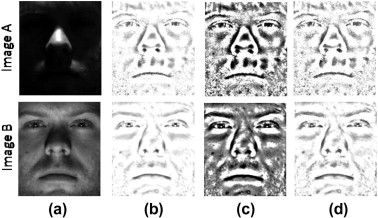
\includegraphics[scale=1]{figures/combination_lbp_gabor} 
\newline

\caption{2 face images of the YaleB face database (a) when processed with Gabor wavelets (b), LBP (c), and Gabor wavelets+LBP (d)\cite{GOH11}}
\label{combination_lbp_gabor}
\end{center} 
\end{figure}

\noindent  LBP has also been combined with the Scale Invariant Feature Transform descriptor (SIFT), which is a ROI descriptor. This descriptor is robust against image rotation, image translations, scaling and lighting variations. Heikkila et al. introduced a combination of the SIFT descriptor with the LBP operator \cite{HEI09}.
\newline
